\documentclass{article}


\usepackage{amsmath} % math stuff
\usepackage{amssymb} % math stuff
\usepackage{array} % equations and stuff
\usepackage{bm} % bold math
%\usepackage{caption} % suppressed table numbering; incompatible with revtex, and longtable, I think
\usepackage{comment} % comment environment
%\usepackage{enumitem} % customization of enumeration, itemize, and description
\usepackage[T1]{fontenc} % font encoding for special characters, must also use scalable font package
\usepackage[margin=0.8in]{geometry} % paper sizes and margins (but be careful not to mess up pre-defined pages)
\usepackage{graphicx} % for graphics
%\usepackage{helvet} % default font is the helvetica postscript font
\usepackage{lipsum} % lorem ipsum filler text
\usepackage{lmodern} % scalable font?
\usepackage{longtable} % multi-page tables
\usepackage{mathrsfs} % math script font
\usepackage{mhchem} % easier chemical formula
\usepackage{microtype} % allows disabling of ligatures
%\usepackage{newcent} % new century schoolbook font
\usepackage{nicefrac}
\usepackage{parskip} % removes paragraph indentation, and adjusts paragraph skip, as well as list items
%\usepackage{setspace} % adjust text spacing and indents
\usepackage{siunitx} % decimal alignment
\usepackage{subfigure} % divided figures
%\usepackage{tabu} % extra table options
\usepackage{textcomp} % symbols
\usepackage{threeparttablex} % better footnotes with longtable
\usepackage{titling} % title placement
\usepackage{ulem} % strikethrough text
%\usepackage{url} % superceded by hyperref
\usepackage{verbatim} % verbatim environment
\usepackage{xcolor} % colors and color boxes
\usepackage{xspace} % commands that don't eat up white space
\usepackage{hyperref} % links and page setup; should always come last

\hypersetup{
	bookmarks=true,
	colorlinks=true,
	citecolor=blue,
	linkcolor=blue,
	urlcolor=blue,
	pdfstartview={XYZ null null 1.0} % default open view is 100%
}

\DisableLigatures[f]{encoding = *, family = * } % disable ff, fi, fl ligatures, without f option, it also disables -- = endash
\renewcommand{\arraystretch}{1} % extra vertical space in tables

\begin{document}

\pagestyle{empty} % don't number pages

% custom title
\begin{center}
{\LARGE Express Riddler}

\vspace{0.15in}

{\Large 17 April 2020}
\end{center}


\section*{Riddle:}

Black Bishop: ``Sir, forensic testing indicates the Queen's assassin, the White Knight between us, has moved exactly eight times since the beginning of the game, which has been played by the legal rules.''

Black King: ``So?''

Black Bishop: ``Well, to convict this assassin, we need to construct a legal game history.
But we just can't figure out how he got there!''

Can you figure it out?

\begin{center}
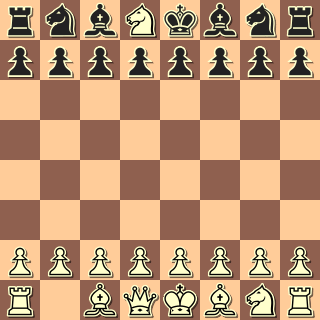
\includegraphics[width=2.5in]{chess.png}
\end{center}

\section*{Solution:}

The trick here is that it seems like there is no solution.
Realizing that there is no solution seems like it might just be the logical trick for which the problem is asking, instead of exhaustively searching for every set of eight moves.
But there is actually a solution.

From the given board, it looks like the white queen's knight is the assassin.
Starting from a white space, however, means that after an even number of moves, the knight must again be on a white space.
But it is actually possible that the assassin is the king's knight, which does start on a black space.
The queen's knight, then, could instead have moved over and taken the other knight's initial position.
This move would have taken an odd number of moves, but it is certainly possible to do.

I show my solution below.
The queen's knight's movements are shown by the blue arrows, and the king's knight's movements by the red arrows.
Of course, going through a legal game means that black must also have made moves at some point.
To remain in its initial setup, though, means that black must have just been moving one or both of its knights back and forth.
Further, looking at the path of the white assassin, black also passed up a chance to capture the knight.
Also, because white would have taken 13 (or any greater odd number) turns, black would have taken 12 or 13 turns also.
With the current setup, it means that black has only taken 12, and so it is currently black's move.

\begin{center}
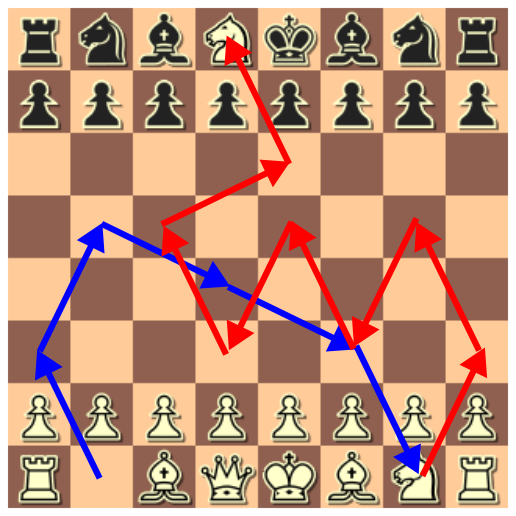
\includegraphics[width=2.5in]{chess2.png}
\end{center}



\end{document}